%%=============================================================================
%% Bijlagen
%%=============================================================================
\chapter{Bijlagen}
\label{ch:bijlagen}

\section{Bijlage 1}
\label{sec:bijlage1}

\subsubsection{Voelde u zich aanwezig op de plaats zelf}
\label{sec:vraag1}
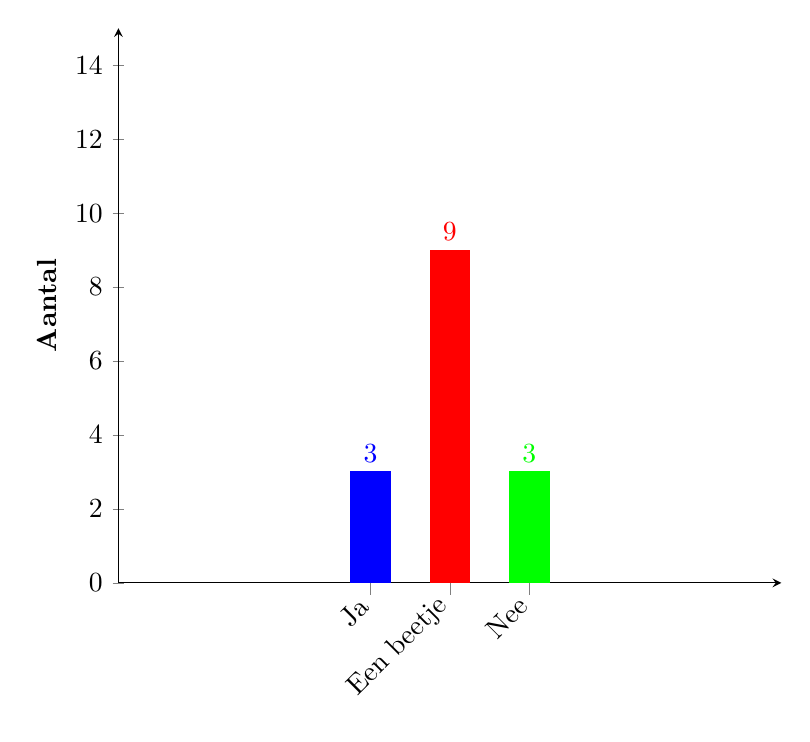
\begin{tikzpicture}
\pgfplotsset{width=10 cm}
\begin{axis} [
symbolic x coords={Ja,Een beetje,Nee},
xtick={Ja,Een beetje,Nee},
x tick label style={rotate=45, anchor=east, align=center},
axis lines=left,
ylabel={\textbf{Aantal}},
legend style={at={(0.5,-0.10)},
	anchor=north,legend columns=1},
ybar=0pt ,
ymin=0,
ymax=15,
samples=2,
domain=1:2,
bar width=0.5cm,                       %% changed
ybar=-0.5cm,                           %% new
enlarge x limits={abs=3.2cm},
nodes near coords,                     %% new 
nodes near coords align={vertical},    %% new
]
\addplot [blue,fill=blue]
coordinates{ (Ja,3) } ;
\addplot [red,fill=red]
coordinates{ (Een beetje,9) } ;
\addplot [green,fill=green]
coordinates{ (Nee,3) } ;


\end{axis}
\end{tikzpicture}

\subsubsection{Vond u de applicatie aangenaam om te gebruiken}
\label{sec:vraag2}
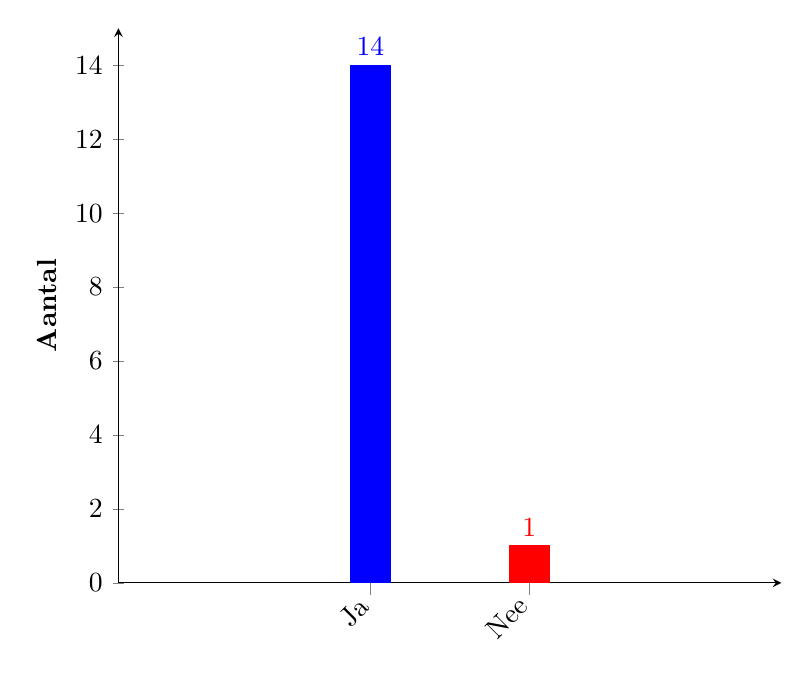
\begin{tikzpicture}
\pgfplotsset{width=10 cm}
\begin{axis} [
symbolic x coords={Ja,Nee},
xtick={Ja,Nee},
x tick label style={rotate=45, anchor=east, align=center},
axis lines=left,
ylabel={\textbf{Aantal}},
legend style={at={(0.5,-0.10)},
	anchor=north,legend columns=1},
ybar=0pt ,
ymin=0,
ymax=15,
samples=2,
domain=1:2,
bar width=0.5cm,                       %% changed
ybar=-0.5cm,                           %% new
enlarge x limits={abs=3.2cm},
nodes near coords,                     %% new 
nodes near coords align={vertical},    %% new
]
\addplot [blue,fill=blue]
coordinates{ (Ja,14) } ;
\addplot [red,fill=red]
coordinates{ (Nee,1) } ;

\end{axis}
\end{tikzpicture}

\subsubsection{Heeft u al eerder gebruik gemaakt van virtual reality?}
\label{sec:vraag3}
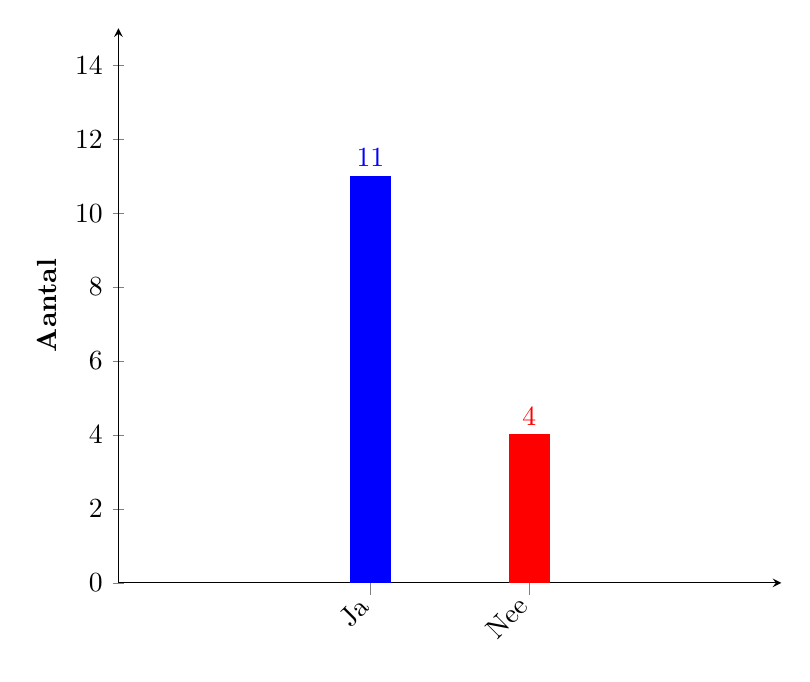
\begin{tikzpicture}
\pgfplotsset{width=10 cm}
\begin{axis} [
symbolic x coords={Ja,Nee},
xtick={Ja,Nee},
x tick label style={rotate=45, anchor=east, align=center},
axis lines=left,
ylabel={\textbf{Aantal}},
legend style={at={(0.5,-0.10)},
	anchor=north,legend columns=1},
ybar=0pt ,
ymin=0,
ymax=15,
samples=2,
domain=1:2,
bar width=0.5cm,                       %% changed
ybar=-0.5cm,                           %% new
enlarge x limits={abs=3.2cm},
nodes near coords,                     %% new 
nodes near coords align={vertical},    %% new
]
\addplot [blue,fill=blue]
coordinates{ (Ja,11) } ;
\addplot [red,fill=red]
coordinates{ (Nee,4) } ;

\end{axis}
\end{tikzpicture}

\subsubsection{Vond u het beeld goed van kwaliteit?}
\label{sec:vraag4}
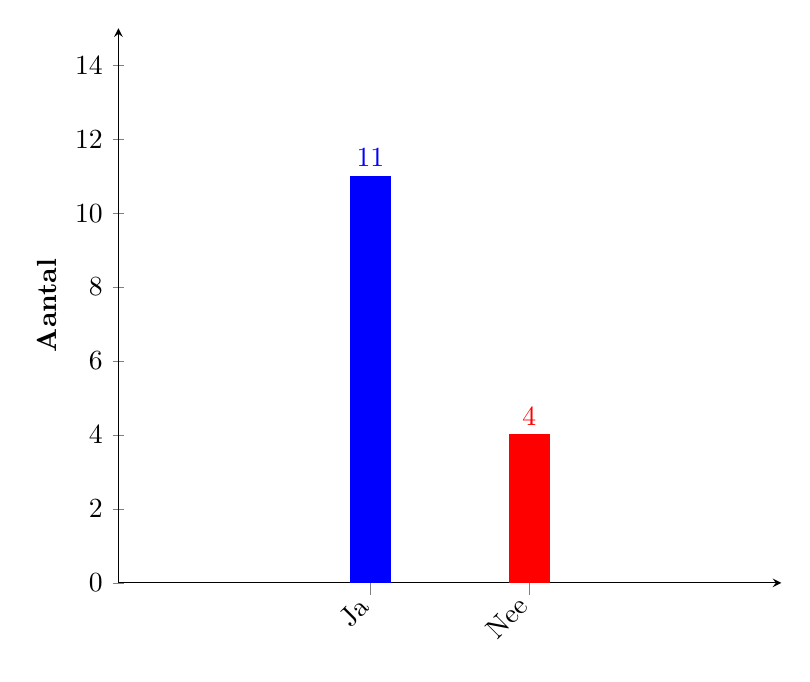
\begin{tikzpicture}
\pgfplotsset{width=10 cm}
\begin{axis} [
symbolic x coords={Ja,Nee},
xtick={Ja,Nee},
x tick label style={rotate=45, anchor=east, align=center},
axis lines=left,
ylabel={\textbf{Aantal}},
legend style={at={(0.5,-0.10)},
	anchor=north,legend columns=1},
ybar=0pt ,
ymin=0,
ymax=15,
samples=2,
domain=1:2,
bar width=0.5cm,                       %% changed
ybar=-0.5cm,                           %% new
enlarge x limits={abs=3.2cm},
nodes near coords,                     %% new 
nodes near coords align={vertical},    %% new
]
\addplot [blue,fill=blue]
coordinates{ (Ja,11) } ;
\addplot [red,fill=red]
coordinates{ (Nee,4) } ;

\end{axis}
\end{tikzpicture}

\subsubsection{Had u last van fysieke ongemakken? (hoofdpijn, duizeligheid, droge ogen, misselijkheid, ...)}
\label{sec:vraag5}
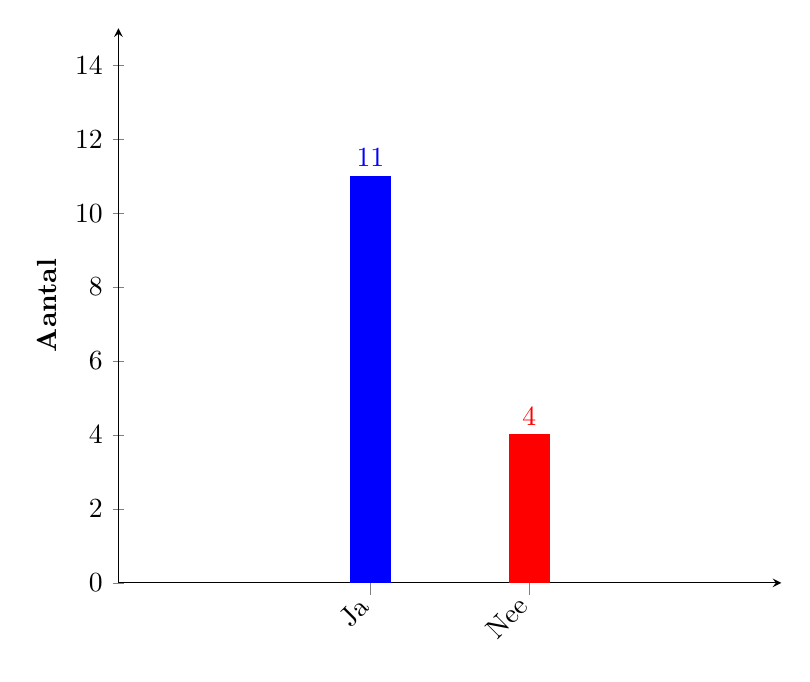
\begin{tikzpicture}
\pgfplotsset{width=10 cm}
\begin{axis} [
symbolic x coords={Ja,Nee},
xtick={Ja,Nee},
x tick label style={rotate=45, anchor=east, align=center},
axis lines=left,
ylabel={\textbf{Aantal}},
legend style={at={(0.5,-0.10)},
	anchor=north,legend columns=1},
ybar=0pt ,
ymin=0,
ymax=15,
samples=2,
domain=1:2,
bar width=0.5cm,                       %% changed
ybar=-0.5cm,                           %% new
enlarge x limits={abs=3.2cm},
nodes near coords,                     %% new 
nodes near coords align={vertical},    %% new
]
\addplot [blue,fill=blue]
coordinates{ (Ja,11) } ;
\addplot [red,fill=red]
coordinates{ (Nee,4) } ;

\end{axis}
\end{tikzpicture}

\subsubsection{Moest u zelf beschikken over zo een headset, zou u dan regelmatig deze soort applicaties gebruiken?}
\label{sec:vraag6}
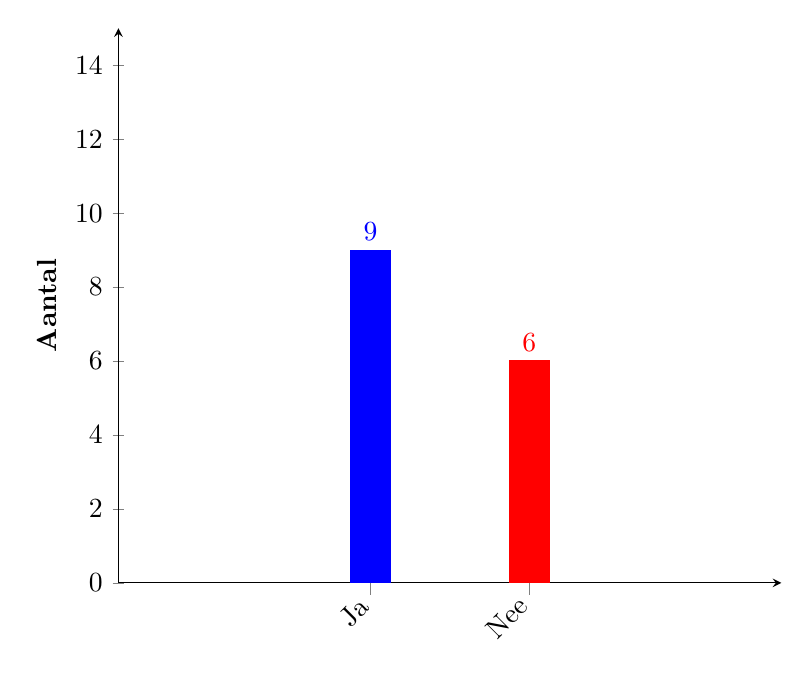
\begin{tikzpicture}
\pgfplotsset{width=10 cm}
\begin{axis} [
symbolic x coords={Ja,Nee},
xtick={Ja,Nee},
x tick label style={rotate=45, anchor=east, align=center},
axis lines=left,
ylabel={\textbf{Aantal}},
legend style={at={(0.5,-0.10)},
	anchor=north,legend columns=1},
ybar=0pt ,
ymin=0,
ymax=15,
samples=2,
domain=1:2,
bar width=0.5cm,                       %% changed
ybar=-0.5cm,                           %% new
enlarge x limits={abs=3.2cm},
nodes near coords,                     %% new 
nodes near coords align={vertical},    %% new
]
\addplot [blue,fill=blue]
coordinates{ (Ja,9) } ;
\addplot [red,fill=red]
coordinates{ (Nee,6) } ;

\end{axis}
\end{tikzpicture}